%!TEX root = ../documentation.tex

\chapter{Norbert - Your StudyBuddy}

\section{Norbert - Wie kommt er das Leben eine Studierenden?}
Norbert - Your StudyBuddy ist eine Anwendung zum Optimieren des Studienalltags, doch wie werden die Studierenden darauf aufmerksam?
Um Norbert bekannt zu machen und die Vorteile der Software zu verbreiten, existieren verschiedene Marketingstrategien die in den nächsten Unterkapiteln vorgestellt werden. Spätestens am ersten Studientag tritt der Studierende über die Kurskennung einem virtuellen Kurs bei und vernetzt sich mit anderen Studierenden des Kurses.

\subsection{Das duale Partnerunternehmen}
Die dualen Partnerunternehmen sind meistens die ersten Anlaufstellen der Studierenden. Im Vorpraktikum wird  - soweit möglich - bei den höheren Semestern nachgefragt, auf welche Aspekte man in den ersten Semestern achten muss. Doch meistens gestaltet dies sich nicht immer als einfach, denn der Austausch von Dokumenten oder ersten ToDo's im neuen Semester, haben sich auch die höheren Semester nicht mehr behalten. Außerdem ist insbesondere in größeren Unternehmen der Austausch aufgrund der komplexeren Unternehmensstruktur erschwert. An diesen Punkten setzt Norbert ein: Das Partnerunternehmen oder die duale Studienvertretung im Unternehmen macht auf die Anwendung aufmerksam. Und kann darüber zentral alle wichtigen Informationen weitergeben. Zudem könnten die Partnerunternehmen als mögliche Hoster der Anwendung in Frage kommen und würden somit die Verwaltung der Anwendung übernehmen.

Jetzt fragt man sich, warum soll eine Firma die Anwendung auf eigene Kosten hosten? Die Antwort ist einfach: Gerade in den ersten Semestern wird das Lernpensum gerne unterschätzt, Aufgaben vergessen, Termine und Fristen nicht eingehalten. Dies führt häufig dazu das bereits nach dem ersten Semester bis zu 50\% der dualen Studierenden ihr Studium abbrechen müssen und das Partnerunternehmen verlassen. Das investierte Geld der Unternehmen ist damit verloren und wichtige zukünftige Mitarbeiter fehlen.

\subsection{Die Duale Hochschule}
Die Duale Hochschule könnte wie die Partnerunternehmen als Hoster der Anwendung in Frage kommen. Durch die Vermarktung der Software auf der DHBW-Webseite oder bei Studieninformationstagen kann bereits früh auf die neue Software aufmerksam gemacht werden. Außerdem stellt eine solche Software für die DHBW ein Alleinstellungsmerksmal dar, da bisher an keiner Hochschule in Deutschland eine solche Softwarelösung existiert. Außerdem können über diese Anwendung wichtige DHBW-Pressemitteilungen schnell und kostengünstig verbreitet werden. Nicht zu verachten ist auch, dass die Möglichkeit besteht, dass die Durchfallquoten der DHBW sinken und dadurch mehr Partnerunternehmen, besser Zuschüsse und ein allgemein höheres Ansehen erzeugt werden kann.

\subsection{Die Studienvertretung} 
Die Studienvertretung kann ähnlich wie die DHBW über die Anwendung über Tagungen, Wahlen, Mitteilungen und Kneipentouren informieren. Durch das Hosting der Anwendung und dem daraus gewonnen Alleinstellungsmerkmal gegenüber anderen Studienvertretungen die eine solche Lösung nicht anbieten, wird das lokale Ansehen gesteigert werden. 

\section{Norbert - Was bietet er?}
Norbert hilft dir deinen Studienalltag besser zu organisieren. Insbesondere werden dabei folgende Funktionen dazu bereitgestellt:
\begin{enumerate}
	\item Automatische Vorschläge zu Aufgaben/ToDo's und automatische Bereitstellung von Informationen
	\item Verwalten von Aufgaben und ToDo's
	\item Anhängen von Dokumenten an ToDo's
	\item Anzeige von Erinnerungen und wichtigen Terminen
	\item Einzigartiger Newsfeed der Aufgaben, ToDo's, Informationen und weitere Aspekte auf einen Blick vereint
	\item Persönliche Kalenderfunktionen in die der Kurskalender mit eingebunden ist
	\item Automatische Extrahierung von Informationen und Dokumenten aus dem Kursverteiler
	\item Bereitstellung von Bahnabfahrtszeiten, Stauinformationen, Mensaplänen
	\item Erinnerungen zum wichtigen Terminen in der Praxisphase (Themeneinreichung, Berichtabgabe uvm.)
	\item uvm.
\end{enumerate}

Die folgende Abbildung verdeutlicht welche Informationen, Termine und Aufgaben der Studierende verpasst haben könnte. Mit Norbert - Your StudyBuddy wäre dies wahrscheinlich nicht passiert.

\newpage
\begin{landscape}
\vspace*{35mm}
	\begin{figure}[H]
	\centering
	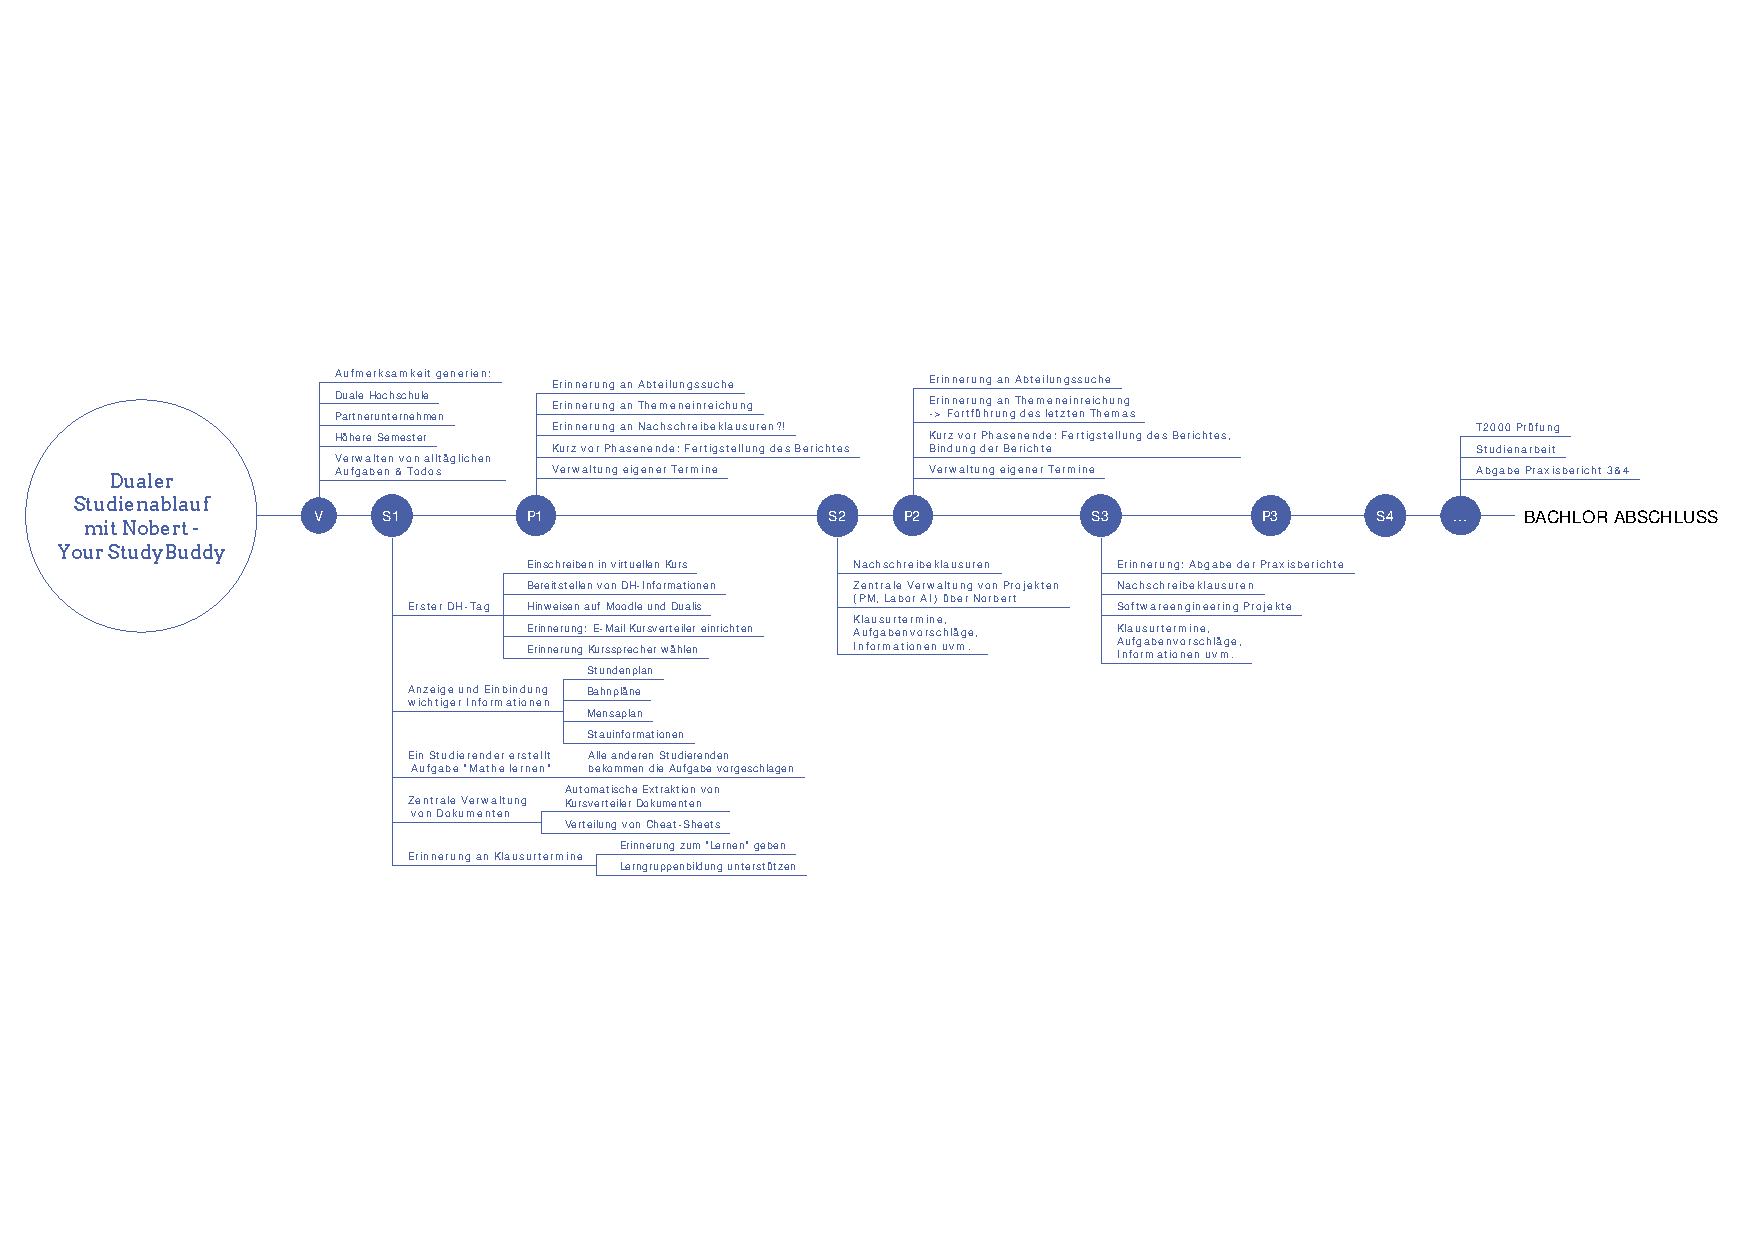
\includegraphics[scale=0.75]{images/timeline.pdf}
	\end{figure}

\end{landscape}

\newpage

\section{Norbert - Wie unterscheidet er sich von anderen Lösungen}